\documentclass[11pt,a4paper]{article}
\usepackage[utf8]{inputenc}
\usepackage[T1]{fontenc}
\usepackage[spanish]{babel}
\usepackage[sfdefault,condensed]{cabin}
\usepackage[margin=2.5cm]{geometry}
\usepackage{graphicx}
\usepackage[hidelinks]{hyperref}
\usepackage[backend=biber,style=ieee]{biblatex}
\addbibresource{referencias.bib}
\setlength{\parindent}{0pt}
\begin{document}
\pagenumbering{roman}
\begin{titlepage}
\centering
{\Large FORM-IC-01\par}
\vspace{1cm}
{\LARGE Plataforma de microservicios de VALORANT\par}
\vspace{1cm}
{\large Byron Daniel Loor Mendoza\par}
\vfill
\textbf{BORRADOR TÉCNICO INCOMPLETO}\par
Estructura sin análisis personal.
% Incorporar los demás datos identificativos solo después de verificarlos.
\end{titlepage}
\pagenumbering{arabic}
\textbf{BORRADOR TÉCNICO INCOMPLETO}
% El análisis personal debe ocupar UNA página, sin carátula ni referencias.
% Comprobar guía, rúbrica, encuadre y restricciones de IA antes de redactar.
\section*{Descripción y escala}
% Byron: redactar desde su lectura y citar con \cite{gunning2020valorant}.
% Distinguir plataforma y servidor de gameplay; fechar las cifras de la fuente.
\section*{Motivos y antecedente}
% Byron: explicar el antecedente sin atribuir una migración monolítica a VALORANT.
\section*{Beneficios y evidencia medible}
% Byron: vincular cada beneficio con evidencia; distinguir simulación y producción.
\section*{Desafíos y soluciones}
% Byron: seleccionar y analizar desafíos y soluciones sustentados por las fuentes.
\section*{Aplicación al PFC y experiencia personal}
% Byron: describir su PFC real, qué tomaría, qué no y por qué.
% Añadir un ejemplo de sistema conocido personalmente, sin inventar experiencia.
\section*{Evidencia de lectura y declaración de IA}
% Las capturas aportadas se incluyen en páginas separadas de evidencia.
% Verificar con la guía la ubicación de la captura y la declaración dentro del límite.
% Declarar herramientas, partes asistidas y verificaciones personales reales.
% Registrar que Codex preparó este esqueleto técnico y sus instrucciones de compilación.
% No afirmar autoría personal de esta estructura ni validaciones no realizadas.
\clearpage
\section*{Evidencias}
\subsection*{1. Interfaz del juego}
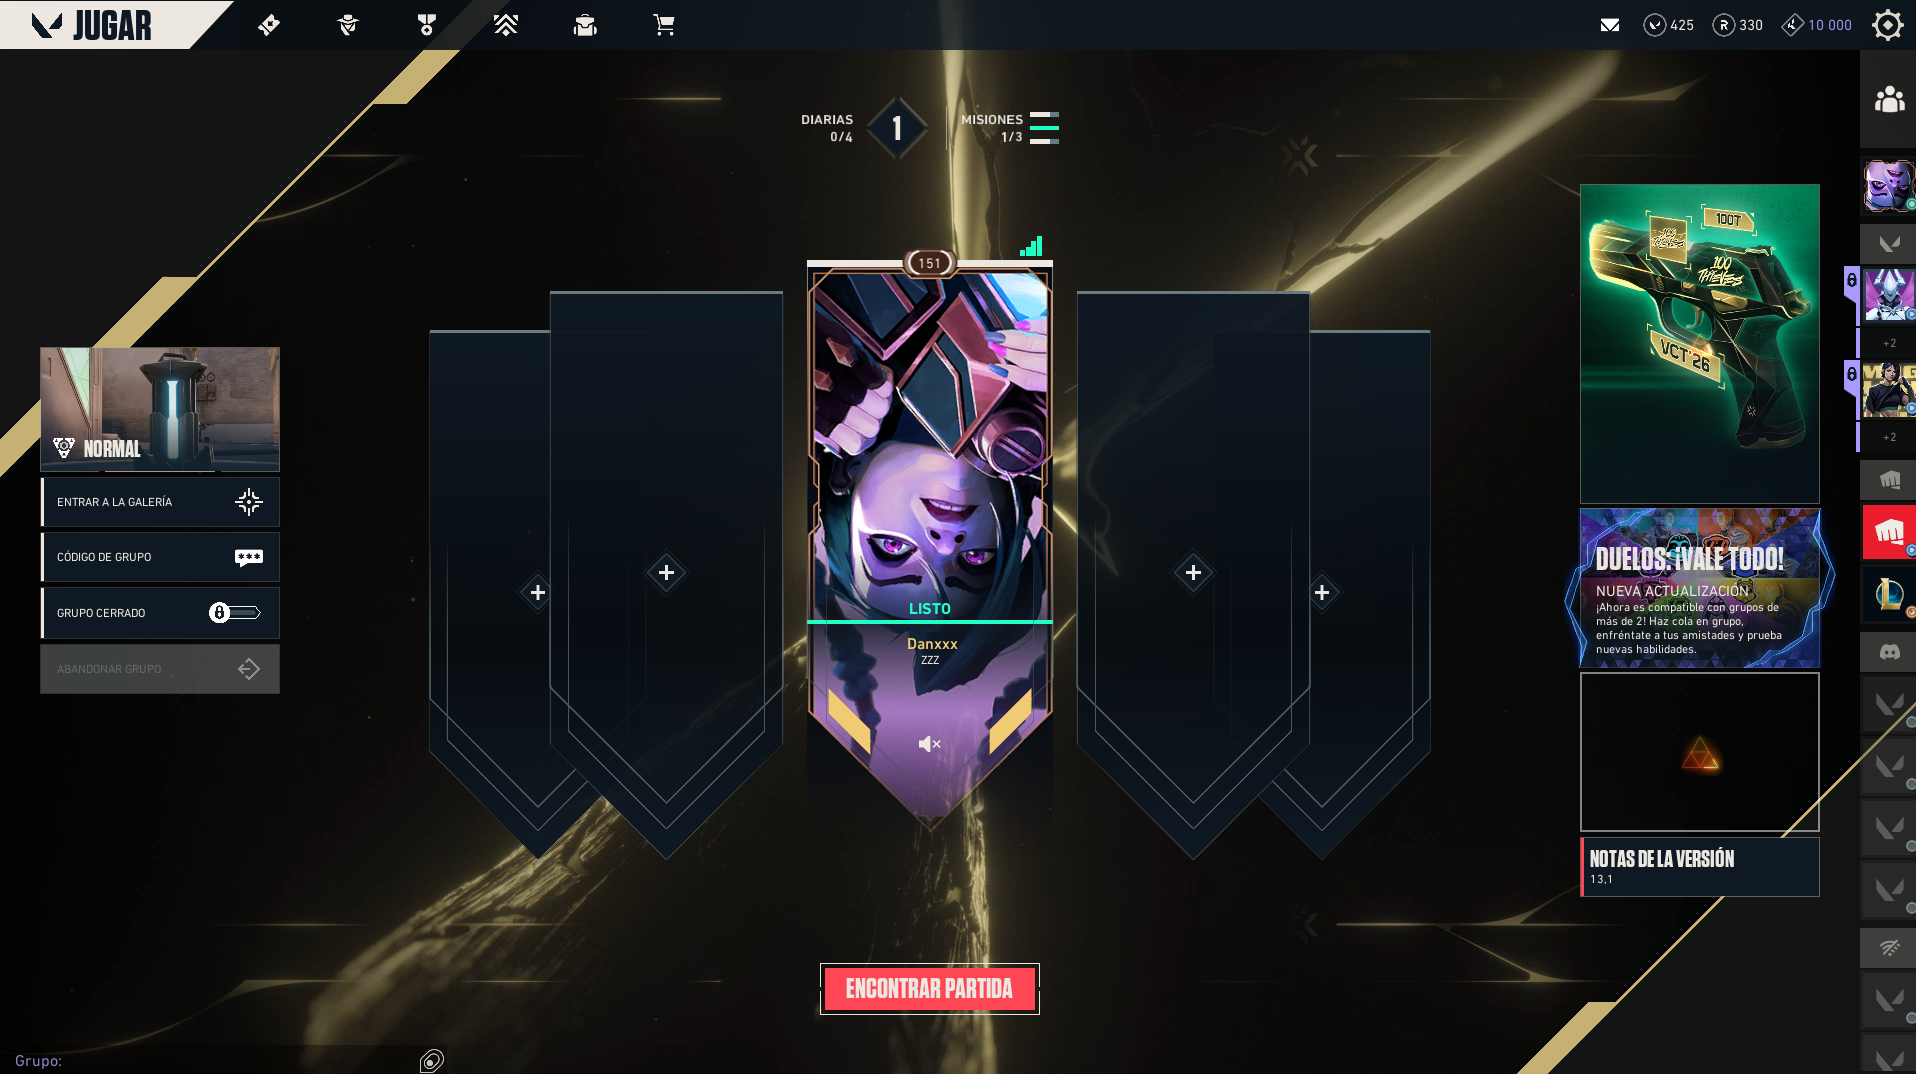
\includegraphics[width=\linewidth]{capturas/01-lobby-valorant.png}

Lobby de VALORANT: interfaz del cliente con el grupo y la opción de encontrar partida.
\clearpage
\section*{Evidencias}
\subsection*{2. Fragmento seleccionado: servicios}
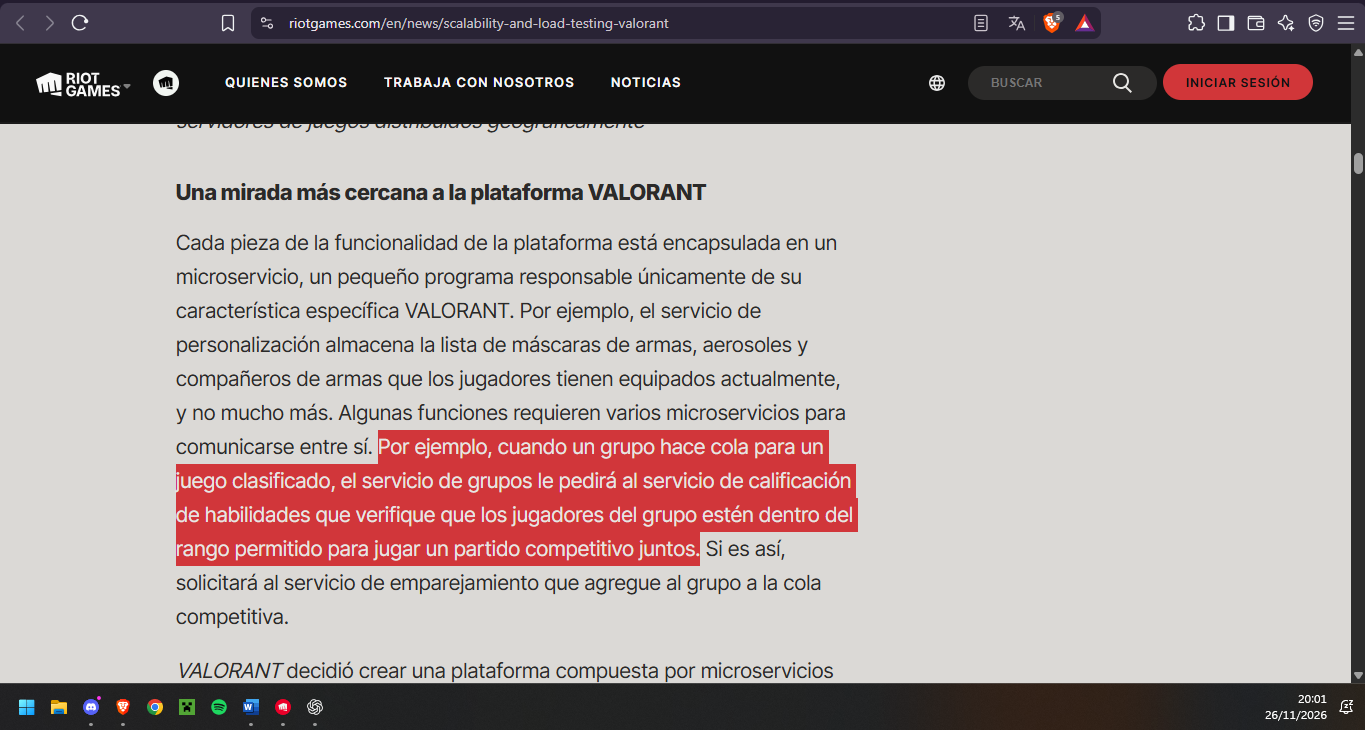
\includegraphics[width=\linewidth]{capturas/02-articulo-servicios.png}

Artículo oficial de Keith Gunning~\cite{gunning2020valorant}, visualizado con traducción del navegador y un fragmento seleccionado en rojo.
\clearpage
\section*{Evidencias}
\subsection*{3. Fragmento seleccionado: antecedente}
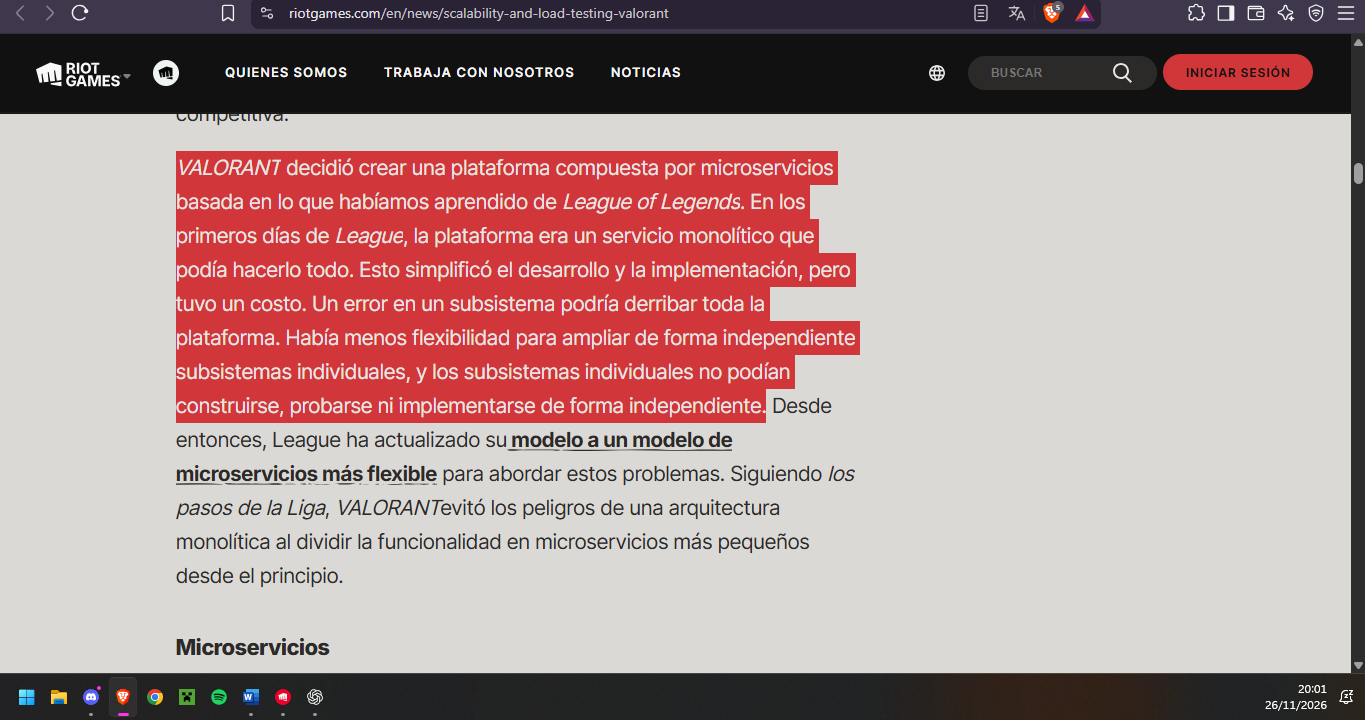
\includegraphics[width=\linewidth]{capturas/03-articulo-antecedente.png}

Artículo oficial de Keith Gunning~\cite{gunning2020valorant}, visualizado con traducción del navegador y un fragmento seleccionado en rojo.
\clearpage
\nocite{gunning2020valorant,hassan2022scalability,aderaldo2025resiliency}
\printbibliography[title={Referencias}]
\end{document}
